%% Copernicus Publications Manuscript Preparation Template for LaTeX Submissions
%% ---------------------------------
%% This template should be used for copernicus.cls
%% The class file and some style files are bundled in the Copernicus Latex Package, which can be downloaded from the different journal webpages.
%% For further assistance please contact Copernicus Publications at: production@copernicus.org
%% https://publications.copernicus.org/for_authors/manuscript_preparation.html

% Force LaTeX to look in current directory first
\makeatletter
\def\input@path{{./}}
\makeatother

%% Please use the following documentclass and journal abbreviations for preprints and final revised papers.

%% 2-column papers and preprints
\documentclass[journal abbreviation, manuscript]{copernicus}


%% Journal abbreviations (please use the same for preprints and final revised papers)


% Advances in Geosciences (adgeo)
% Advances in Radio Science (ars)
% Advances in Science and Research (asr)
% Advances in Statistical Climatology, Meteorology and Oceanography (ascmo)
% Aerosol Research (ar)
% Annales Geophysicae (angeo)
% Archives Animal Breeding (aab)
% Atmospheric Chemistry and Physics (acp)
% Atmospheric Measurement Techniques (amt)
% Biogeosciences (bg)
% Climate of the Past (cp)
% DEUQUA Special Publications (deuquasp)
% Earth Surface Dynamics (esurf)
% Earth System Dynamics (esd)
% Earth System Science Data (essd)
% E&G Quaternary Science Journal (egqsj)
% EGUsphere (egusphere) | This is only for EGUsphere preprints submitted without relation to an EGU journal.
% European Journal of Mineralogy (ejm)
% Geochronology (gchron)
% Geographica Helvetica (gh)
% Geoscience Communication (gc)
% Geoscientific Instrumentation, Methods and Data Systems (gi)
% Geoscientific Model Development (gmd)
% History of Geo- and Space Sciences (hgss)
% Hydrology and Earth System Sciences (hess)
% Journal of Bone and Joint Infection (jbji)
% Journal of Environmentally Compatible Air Transport System (jecats)
% Journal of Micropalaeontology (jm)
% Journal of Sensors and Sensor Systems (jsss)
% Magnetic Resonance (mr)
% Mechanical Sciences (ms)
% Natural Hazards and Earth System Sciences (nhess)
% Nonlinear Processes in Geophysics (npg)
% Ocean Science (os)
% Polarforschung - Journal of the German Society for Polar Research (polf)
% Proceedings of the International Association of Hydrological Sciences (piahs)
% Proceedings of the International Ocean Drilling Programme (piodp)
% Safety of Nuclear Waste Disposal (sand)
% Scientific Drilling (sd)
% SOIL (soil)
% Solid Earth (se)
% State of the Planet (sp)
% The Cryosphere (tc)
% Weather and Climate Dynamics (wcd)
% Web Ecology (we)
% Wind Energy Science (wes)


%% \usepackage commands included in the copernicus.cls:
%\usepackage[german, english]{babel}
%\usepackage{tabularx}
%\usepackage{cancel}
%\usepackage{multirow}
%\usepackage{supertabular}
%\usepackage{algorithmic}
%\usepackage{algorithm}
%\usepackage{amsthm}
%\usepackage{float}
%\usepackage{subfig}
%\usepackage{rotating}
\usepackage{bm}
\usepackage{amsmath}
\DeclareMathOperator*{\argmax}{arg\,max}
\DeclareMathOperator*{\argmin}{arg\,min}

% ---- Custom commands ----
\newcommand\todo[1]{\textbf{\textcolor{red}{TODO: #1}}}   % define \todo{}
\newcommand\note[1]{\textbf{\textcolor{blue}{NOTE: #1}}}   % define \note{}


\begin{document}

\title{Sensitivity of Antarctic sea level contribution to regularisation of the initialising inverse problem}

% \Author[affil]{given_name}{surname}

\Author[1][jonathan.barnsley@kcl.ac.uk]{Jonathan R}{Barnsley} %% correspondence author
\Author[1]{Tamsin L}{Edwards}
\Author[1]{Alex}{Bradley}
\Author[2]{Stephen L}{Cornford}
\Author[2]{Matt}{Trevers}

\affil[1]{King's College London, Department of Geography, London, UK}
\affil[2]{University of Bristol, Department of Geography, Bristol, UK}

%% The [] brackets identify the author with the corresponding affiliation. 1, 2, 3, etc. should be inserted.

%% If an author is deceased, please add \deceased[$Deceased date if applicable$]{$Author number$} (e.g. \deceased[13 November 2015]{2}) at the end of the affiliations. The author number depends on the placement of the author in the author list, e.g. the third author has number 3.


%% If authors contributed equally, please add \equalcontrib{$Author numbers$} (e.g. \equalcontrib{1,3}) at the end of the affiliations. The author number depends on the placement of the author in the author list, e.g. the third author has number 3.

\runningtitle{Sensitivity of Antarctic sea level contribution to initialisation choices in the BISICLES ice sheet model}

\runningauthor{Barnsley et al.}





\received{}
\pubdiscuss{} %% only important for two-stage journals
\revised{}
\accepted{}
\published{}

%% These dates will be inserted by Copernicus Publications during the typesetting process.


\firstpage{1}

\maketitle

\begin{abstract}
The ice sheet initial state is known to be a significant source of uncertainty in future sea level contribution, but this uncertainty is rarely explored outside of large-scale model intercomparison projects. Century-scale projections of the Antarctic Ice Sheet commonly generate an initial state by solving an inverse problem for basal friction and ice stiffness such that modelled surface ice velocities closely match observations. However, inverse problems are ill-posed and can absorb errors originating elsewhere in the model, for example in the bed topography or unresolved physics. While this yields realistic short-term behaviour, it may undermine the accuracy of long-term projections.

Here, we quantify how choices made in the inverse problem influence Antarctica's multi-century sea level contribution. Using the BISICLES ice sheet model, we generate an ensemble of initial states by perturbing two regularisation parameters, which control the smoothness of inferred basal friction and ice stiffness. We then project them forward to 2300 under both low and high emission scenarios. We find that sensitivity to regularisation of the ice-stiffness field is comparable to other commonly perturbed parameters on a century timescale but declines on longer timescales, whereas sensitivity to friction regularisation is consistently small — much lower than reported for an equivalent study of the Amundsen Sea Embayment. Our results suggest that the importance of these initialisation choices for sea level projections may depend on the model, domain, resolution, or timescale considered.

\end{abstract}


%\copyrightstatement{} %% This section is optional and can be used for copyright transfers.


\introduction%% \introduction[modified heading if necessary]

The Antarctic Ice Sheet is the largest potential contributor to sea level rise, but its response to ongoing and future climate change remains highly uncertain \citep{fox-kemperOceanCryosphereSea2021}. This uncertainty is even more pronounced on timescales spanning multiple centuries, with projections to 2300 under high emissions ranging from near-zero to multiple metres of sea level contribution \citep{golledgeMultimillennialAntarcticCommitment2015,bulthuisUncertaintyQuantificationMulticentennial2019,decontoParisClimateAgreement2021,greveFutureProjectionsAntarctic2023,seroussiEvolutionAntarcticIce2024,coulonShorttermUncertaintiesLongterm2025}. Quantifying uncertainty in the timing and magnitude of sea level rise is important for climate adaptation strategies such as sea defenses, and underestimating uncertainty poses a risk to the resilience of coastal communities \citep{hinkelMeetingUserNeeds2019,koppUsableScienceManaging2019}. Ice sheet modelling studies that seek to produce usable projections of future sea level rise should therefore make efforts to include the dominant sources of uncertainty.

Uncertainty in the output of ice sheet models can be decomposed into parametric uncertainty, uncertainty in the climate forcing, and model structural uncertainty, which itself encompasses the form of parameterisations, the stress-balance approximation, the initial state, and much more. Most commonly, studies will consider uncertainty in the climate forcing, either by selecting numerous emission scenarios, climate models, or else through a climate indexing method \citep[e.g.][]{decontoParisClimateAgreement2021,greveFutureProjectionsAntarctic2023}. Increasingly, studies are sampling a wide range of uncertain model parameters and parameterisations \citep{bulthuisUncertaintyQuantificationMulticentennial2019,hillQuantifyingPotentialFuture2021,coulonDisentanglingDriversFuture2024,coulonShorttermUncertaintiesLongterm2025,rosierCalibratedSeaLevel2025}. Model structural uncertainty, whilst touched on by some of these studies \citep[notably][]{coulonShorttermUncertaintiesLongterm2025}, is largely explored through international projects such as the Ice Sheet Model Intercomparison Project \citep[ISMIP6,][]{nowickiIceSheetModel2016}, and is the largest source of uncertainty in those experiments \citep{seroussiInsightsVulnerabilityAntarctic2023}. The InitMIP branch of ISMIP6 was designed to specifically isolate uncertainty in the ice sheet initial state, showing that projected sea level contribution is highly sensitive to the choice of initialisation \citep{seroussiInitMIPAntarcticaIceSheet2019}. However, outside of these large intercomparison projects, uncertainty in the ice sheet initial state is less well-explored, since producing multiple realistic initial states is often time consuming and computationally expensive.

The initial state refers to a set of spatial fields defining the physical condition of the ice sheet, which can include ice thickness, bedrock elevation, ice temperature or enthalpy, basal properties, damage, and others. Ideally, these would be similar to the modern ice sheet whilst producing short-term behaviour that resembles observed trends. However, this is not straightforward to achieve, mainly due to inconsistencies between datasets and the model physics. Initialisation methods that approach this problem can be broadly divided into two philosophies: model spin-ups and data assimilation, although some approaches combine elements of both \citep{pollardSimpleInverseMethod2012,leclechRapidlyConvergingInitialisation2019}. Here, we focus only on initialisation through data assimilation, which accounted for 7 of the 25 submissions to initMIP.\@ Based on early work by~\cite{macayealBasalStressDistribution1992}, this typically solves an inverse problem for basal friction and ice rheology parameters such that modelled ice velocities closely match observations. Approaches of this kind have been implemented into numerous ice sheet models and applied to the Antarctic Ice Sheet or its basins \citep{morlighemInversionBasalFriction2013,gagliardiniCapabilitiesPerformanceElmer2013,cornfordCenturyscaleSimulationsResponse2015,arthernFlowSpeedAntarctic2015,hoffmanMPASAlbanyLandIce2018,rosierCalibratedSeaLevel2025}. Inverse methods can produce initial states with very good fits to observed dynamics. However, they are also ill-posed in that the data does not uniquely constrain the solution. Other equally plausible solutions to the inverse problem could yield different future sea level outcomes, but these are rarely explored. Furthermore, inverse problems can introduce compensating errors for deficiencies elsewhere in the model, which then influence future mass loss when the model is projected forward \citep{berendsCompensatingErrorsInversions2023}.

Standard approaches to the inverse problem minimise a loss function comprised of a model-observation misfit and regularisation term. This yields a single best estimate but gives no information about its associated uncertainty. For this, one would need to know the local curvature of the loss function about its minimum, which is described by the Hessian matrix. For practical ice sheet modelling purposes, the Hessian is too large to compute directly, but can be approximated via its low-rank structure \citep{petraComputationalFrameworkInfiniteDimensional2014}. The resulting problem is still expensive to solve, but has allowed for the local approximation of the posterior distribution in idealised ice sheet problems \citep{petraComputationalFrameworkInfiniteDimensional2014,babaniyiInferringBasalSliding2021} or small realistic domains \citep{gopalanBayesianInferenceIce2021,brinkerhoffVariationalInferenceGlacier2022}.~\cite{isaacScalableEfficientAlgorithms2015} perform a Bayesian inversion for basal friction over the Antarctic ice sheet by further assuming that the posterior is locally Gaussian about the optimal solution (equivalently: the loss function is locally quadratic). However, this may not translate well to inverse problems that solve for both friction and rheology, since non-uniqueness of the solution could produce posterior geometry that is poorly represented by a Gaussian approximation. A Bayesian inversion for both friction and rheology has yet to be completed at a continent scale, motivating alternative methods that do not sample from the posterior, but nonetheless explore uncertainty in the solution to the inverse problem. The simplest approach is to produce an ensemble of projections in which the solved fields from a single inversion are variably scaled by a uniform multiplier \citep[e.g.][]{niasContrastingModelledSensitivity2016,bevanAmundsenSeaEmbayment2023}. These studies then downweight ensemble members with poor fits to observed dynamics using a post-hoc calibration. However, this only allows for uniform scaling and leaves the spatial pattern unchanged. Some studies perturb the bedrock elevation and solve inverse problems for each realisation \citep{werneckeQuantifyingImpactBedrock2022,krishnaQuantifyingUncertaintyGreenlands2026}, though care must be taken to account for spatially autocorrelated errors in the topography dataset. A third approach is to treat hyperparameters within the inversion as uncertain parameters and perturb these in a traditional uncertainty quantification framework \citep{rosierCalibratedSeaLevel2025}. This allows for spatially-varying perturbations that are physically plausible by design.

Methods to solve the inverse problem vary between models \citep[see e.g.][]{barnesTransferabilityAdjointInversion2021}, but most rely on some form of regularisation. If unregularised, the optimisation introduces short-wavelength, high-amplitude variability into the inferred fields, which overfit to noisy errors in the observed velocity. Regularisation imposes structure on the solution by penalising roughness and encouraging smooth solutions. However, the strength of regularisation is left largely up to the discretion of the user. An L-curve heuristic is commonly used to justify a choice of regularisation strength by finding the optimal compromise between solution fit and smoothness, characterised by the corner of the `L' \citep{hansenAnalysisDiscreteIllPosed1992}. This does not guarantee, however, that the corner of the L-curve corresponds to anything physically meaningful, nor that the resulting fields are representative of real basal and rheological properties. The location of the L-curve corner has also been shown to depend on choices such as mesh resolution and parameterisations, which complicates its use as an objective criterion \citep{wolovickRegularizationLcurvesIce2023}. Furthermore,~\cite{rosierCalibratedSeaLevel2025} demonstrate that projected sea level contribution from the Amundsen Sea Sector can be highly sensitive to regularisation in the inverse problem as formalised by the \'Ua ice sheet model. This suggests that regularisation hyperparameters may be a route to exploring uncertainty in sea level projections arising from the inverse problem --- and, by association, the initial state --- but it is not yet clear how this result translates to other models or domains.

To further study uncertainties associated with the inverse problem, we use the BISICLES ice sheet model to assess the sensitivity of Antarctic sea level contribution to regularisation parameters in the inverse problem. We produce an ensemble of initial states by perturbing these parameters, alongside other commonly perturbed ice sheet model parameters, and project them forward to 2300 under a high-emission scenario. We find that regularisation parameters can be a moderate source of uncertainty in century-scale sea level projections, but that this sensitivity is likely not consistent across models, domains, and timescales. We discuss the implications of these results for future research efforts to explore initial state uncertainty in sea level projections.

\section{Methods}
\subsection{BISICLES ice sheet model}

BISICLES \citep{cornfordAdaptiveMeshFinite2013} is a finite volume, vertically integrated ice sheet model, which has been used extensively for century-scale modelling of the Antarctic Ice Sheet \citep{cornfordCenturyscaleSimulationsResponse2015,niasAssessingUncertaintyDynamical2019,sunAntarcticIceSheet2020,werneckeQuantifyingImpactBedrock2022,siahaanAntarcticContribution21stcentury2022,oneillISMIP6basedAntarcticProjections2025}. It uses the L1L2 approximation to Stokes flow \citep{schoofThinFilmFlowsWall2010}, which incorporates membrane stresses with a simplified treatment of vertical shear, allowing it to simulate a wide range of flow regimes in Antarctica with computational efficiency. It also features an adaptive mesh, which refines mesh resolution close to the grounding line and in regions of fast flow. Here, we run BISICLES with a base resolution of 8 km and 3 levels of refinement, up to a finest resolution of 1 km. This significantly improves the representation of grounding line dynamics compared to coarser grids \citep{cornfordAdaptiveMeshRefinement2016}.

BISICLES solves the 2-dimensional L1L2 mass transport and stress balance equations outlined in \citet{cornfordCenturyscaleSimulationsResponse2015}. They feature a vertically integrated effective viscosity, $\phi h \bar{\mu}$, defined by:
\begin{equation}
    \phi h \bar{\mu}(x, y) = \phi \int_{s-h}^{s} \mu(x, y, z) dz,
\end{equation}

\noindent where $h$ is ice thickness, $s$ is surface elevation, and $\phi$ is an uncertain, spatially-varying coefficient that is determined by the inverse problem. Values of $\phi < 1$ correspond to softening of the ice and values $\phi > 1$ to strengthening, with a default value $\phi = 1$. The vertically varying effective viscosity, $\mu(x, y, z)$,  is calculated using Glen's flow law \citep{glenCreepPolycrystallineIce1955}:
\begin{equation}
    \mu(x, y, z) = \frac{1}{2 A_0 A(T) \tau^{n-1}},
\end{equation}

\noindent where $A(T)$ is a temperature-dependent Paterson rate factor \citep{cuffeyPhysicsGlaciers2010}, $\tau$ is the effective deviatoric stress, and the flow law exponent $n$ is an uncertain parameter that we perturb in our experiment. The 3-dimensional temperature field is derived from a 100,000-year thermal spin-up described in \citet{treversRetreatThwaitesGlacier2024}. Previous studies have perturbed $n$ after model initialisation by scaling $A(x, y)$ to ensure that the effective viscosity is unchanged everywhere \citep{getraerIncreasingGlenNye2025,rosierCalibratedSeaLevel2025}. However, we follow \citep{martinRatesSeaLevelRise2026} by fixing $n$ before initialisation and introducing a spatially-uniform correction factor, $A_0 = 100,000^{(3-n)}$ to ensure that the effective viscosity is independent of $n$ at a reference stress of 100 kPa. Either side of this value, the flow law diverges from the $n=3$ case, but the effective viscosity is scaled by $\phi$ during the inverse problem so that the initial state matches observed ice velocities.

Basal sliding is governed by a regularised-Coulomb sliding law, which smoothly transitions between Weertman and Coulomb behaviour near to a reference velocity $u_0$ = 300 m a$^{-1}$ \citep{joughinRegularizedCoulombFriction2019}. As such, the slow-moving ice sheet interior stays in a power-law regime, whilst fast-flowing ice streams aproach the perfectly plastic sliding limit. The basal shear stress, $\bm{\tau}_b = -\alpha \mathbf{u}_b$, is given by:
\begin{equation}\label{eq:friction_law}
    \alpha = C \, \lvert \mathbf{u}_b \rvert^{\,m-1}
         \left( \frac{\lvert \mathbf{u}_b \rvert}{u_0} + 1 \right)^{-m},
\end{equation}

\noindent where the friction exponent $m$ is an uncertain parameter that we perturb in our experiment and $C$ is a spatially-varying friction coefficient that is also determined by the inverse problem. The form in~\eqref{eq:friction_law} is equivalent to~\cite{joughinRegularizedCoulombFriction2019} with $m \rightarrow 1/m$ and $C \rightarrow Cu_0^m$, giving C the same units as in the standard power law. This performs similarly to other commonly used sliding laws for key glaciers in Antarctica \citep{barnesPredictivePowerIce2022}.

\subsection{Model initialisation}

We initialise BISICLES using an inverse method to solve for the basal friction coefficient, $C$, and the viscosity coefficient, $\phi$, such that modelled surface velocities closely match observations. BISICLES uses conjugate gradient descent \citep{10.5555/865018} to minimise a cost function, $J$, defined by:
\begin{equation}
    J = J_{m} + J_{p},
\end{equation}

\noindent where $J_m$ is a function of the velocity misfit
\begin{equation}
    J_m = \frac{1}{2} \int_{\Omega_V} {\left( |\mathbf{u}| - |\mathbf{u}_{obs}| \right)}^2 d\Omega_V,
    \label{eq:misfit_function}
\end{equation}

\noindent and $J_p$ is a Tikhonov penalty function
\begin{equation}
    J_p = \frac{\alpha_C}{2}  \int_{\Omega_V} {|\nabla C|}^2 d\Omega_V + \frac{\alpha_{\phi}}{2}  \int_{\Omega_V} {|\nabla \phi|}^2 d\Omega_V,
\end{equation}

\noindent where $\alpha_C$ and $\alpha_{\phi}$ are regularisation parameters that respectively control the smoothness of $C$ and $\phi$, $\Omega_V$ is the domain over which velocities are observed, and $\mathbf{u}_{obs}$ are the surface velocities from \citet{rignotMEaSUREsInSARBasedAntarctica2017}. In our experiment, we treat both $\alpha_C$ and $\alpha_{\phi}$ as uncertain parameters within a range of values (Section~\ref{sec:experiment_design}). % determined by L-curve analysis (Appendix~\ref{sec:l-curves})

We solve the inverse problem using a linear sliding law ($\bm{\tau}_b = -C_1\mathbf{u}_b$) to simplify the stress balance, although this does come with a trade-off of more rounded, less well-defined L-curve corners \citep{wolovickRegularizationLcurvesIce2023}. We then adjust $C$ post-inversion such that basal drag (and therefore ice velocity) remains unchanged. This is done by scaling $C$ over grounded ice such that
\begin{equation}
    C_{m} = C_1 \lvert \mathbf{u} \rvert^{1-m} \left( \frac{\lvert \mathbf{u} \rvert}{u_0} + 1 \right)^m.
\end{equation}

\noindent Here, a minimum of 1 ma$^{-1}$ is applied over $\lvert \mathbf{u}(x, y) \rvert$ to avoid unrealistically high friction in regions of very slow flow. This has the drawback that the initial velocity of ice in regions with $\lvert \mathbf{u} \rvert \ll 1$ may no longer be an optimal fit to observations, but only occurs in regions in which the observed velocity already poorly constrains basal friction \citep{isaacScalableEfficientAlgorithms2015}. The initial ice geometry is taken from BedMachine Antarctica v3 \citep{morlighemMEaSUREsBedMachineAntarctica2022}, the initial guess for $\phi$ is uniformly 1, and the initial guess for $C$ is calculated by equating basal drag to the driving stress. This yields
\begin{equation}
    C_{init} = \rho_i g h \lvert \nabla s \rvert \lvert \mathbf{u} \rvert^{-1},
\end{equation}

\noindent where $\rho_i = 917$ kg m$^{-3}$ is the density of ice and $g = 9.81$ m s$^{-2}$ is gravitational acceleration. As is common with initialisation by inverse problem, we observe a short-term shock immediately after initialisation as the model adjusts to inconsistencies between the geometry and model physics. We therefore allow a 15-year relaxation period, during which we periodically re-solve the inverse problem each year following~\cite{bevanAmundsenSeaEmbayment2023}. Throughout the relaxation, the thickness of floating ice shelves is held constant and we apply a constant background surface mass balance, derived by taking the 1980--2021 mean surface mass balance from a simulation by the MAR regional climate model, forced by ERA5-Interim data \citep{agostaEstimationAntarcticSurface2019} \note{I got this dataset from Matt --- Matt, do you know if this is the correct citation and have I described this correctly? Because Agosta et al. only seems to go up to 2015}. In total, we generate 7 initial states for our experiment by perturbing parameters used within the initialisation (see Section~\ref{sec:experiment_design}). These are then projected forward under a climate forcing described in Section~\ref{sec:forcing}.

\subsection{Climate forcing}\label{sec:forcing}
% Inverse methods produce a good fit to observed velocities, but this often results in poor fits to other measurables such as the rate of elevation change, $\dot{h}$. We could incorporate an additional term into the cost function (\ref{eq:misfit_function}) to improve the fit to $\dot{h}$, but this would come at a cost to the velocity misfit. Model outputs can also be very sensitive to the balance between the velocity and $\dot{h}$ components of a misfit function \citep{rosierCalibratedSeaLevel2025}. Instead, we choose to correct for bias in $\dot{h}$ by exploiting uncertainty in the surface mass balance SMB. We apply a background rate of surface mass balance that is designed to bridge the gap between modelled and observed $\dot{h}$:
% \begin{equation}
%     \mathrm{SMB}_{bkg} = \dot{h}_{obs} + \nabla \cdot \left( \mathbf{u} h \right)
% \end{equation}

% \noindent where $\dot{h}_{obs}$ is the observed rate of elevation change from \citep{smithPervasiveIceSheet2020} and $\nabla \cdot \left( \mathbf{u} h \right)$ is the flux divergence at the end of a relaxation with default parameter values. We set bounds of -1--2 ma\textsuperscript{-1} and apply a Gaussian filter to smooth out short-wavelength components of the flux divergence \citep{niasContrastingModelledSensitivity2016}. The beneficial effect of this is to correct a thickening bias over the Antarctic Peninsula and trans-Antarctic mountains, where our 1 km grid resolution is too coarse to resolve the dynamics of these smaller glaciers. However, the resulting surface mass balance is purely synthetic and a poor representation of reality. Nonetheless, it corrects the significant model drift that occurs over multiple centuries without the need for a control simulation. We therefore consider it to be adequate for the purposes of a sensitivity study.

Following initialisation, we apply a time-varying surface and basal mass balance between an initial date in 2007 until 2300. The surface mass balance is composed of the background rate used in the relaxation, upon which we apply anomalies derived from the CESM2-WACCM climate model \citep{danabasogluCommunityEarthSystem2020} under the SSP5-8.5 emissions scenario \citep{meinshausenSharedSocioeconomicPathway2020}. The anomalies are annual means with respect to the 1995--2014 climatology, calculated by subtracting evaporation, sublimation and runoff from precipitation, as in \citep{nowickiExperimentalProtocolSea2020}. CESM2-WACCM was chosen for its strong climate forcing to maximise the signal-to-noise ratio in our results, but its high climate sensitivity and the aggressive increase in emissions in SSP5-8.5 mean it is not necessarily representative of the most likely future climate \citep{hausfatherAssessmentCurrentPolicy2025}. \todo{ref for CESM2 climate sensitivity}

To compute a basal mass balance, we follow the method described by~\cite{jourdainProtocolCalculatingBasal2020b}, using the non-local quadratic parameterisation of ice shelf basal melt with respect to ocean thermal forcing.
\begin{align}
    m(x, y) &= \gamma_0 \times {\left( \frac{\rho_{\text{sw}}c_{\text{pw}}}{\rho_\text{i} L_\text{f}} \right)}^2 \\ 
    &\times {\left( \text{TF}(x, y, z_{\text{draft}}) + \delta T_{\text{sector}} \right)} \\ 
    &\times |{\langle \text{TF} \rangle_{\text{draft} \in \text{sector}}} + \delta T_{\text{sector}}|,
\end{align}

\noindent where $\rho_{\text{sw}}$ and $c_{\text{pw}}$ are the density and specific heat capacity of seawater, $\rho_\text{i}$ is the density of ice, $L_\text{f}$ is the latent heat of fusion, and $\gamma_0$ is the ice-ocean heat flux. $\text{TF}(x, y, z_{\text{draft}})$ is the ocean thermal forcing anomaly at the depth of the ice shelf draft, calculated from ocean temperature and salinity outputs from CESM2-WACCM.\@ Anomalies are calculated with respect to the initial thermal forcing such that basal mass balance is zero upon initialisation. Whilst this underestimates present-day melt rates in some key regions \citep{adusumilliInterannualVariationsMeltwater2020}, any errors are quickly outweighed by the strong climate forcing in SSP5-8.5 and we consider it to be adequate for the purposes of a sensitivity study. $\delta T_{\text{sector}}$ is a sector-specific offset used by~\cite{jourdainProtocolCalculatingBasal2020b} to fit basal melt to observed rates. However, our anomaly approach significantly reduces the impact of this term and we fix it constant at the `MeanAnt' median-calibrated values derived by~\cite{jourdainProtocolCalculatingBasal2020b}.

\subsection{Experiment design}\label{sec:experiment_design}

We assess sensitivity to parameters through a simple `axial' ensemble, in which we perturb one parameter at a time to a given upper or lower bound whilst holding all other parameters at their chosen nominal value (Table~\ref{tab:parameters}). A method suggested by~\cite{wolovickRegularizationLcurvesIce2023} chooses a suitable range of regularisation values by considering the points at which L-curve curvature has dropped to a half of its maximum value (the maximum occuring at the L-curve corner). However, the authors note that the choice of a half is arbitrary and that the upper bound in particular is highly sensitive to this choice. In the interest of sampling the widest possible uncertainty, we instead choose an upper and lower bound based on separate criteria: the lower bound is selected such that lower values of regularisation no longer improve the misfit (the solution is essentially unregularised); the upper bound corresponds to a solution which offers no (or marginal) improvement to the misfit over the initial guess. Note that, for $C$, this does not mean that the solution is equal to the driving stress, since smoother solutions can still improve the misfit. However, for $\phi$, this results in a solution that is near-uniformly 1. This level of regularisation is well beyond the level suggested by L-curve heuristics, but represents a case in which the model's inability to capture processes normally absorbed by $\phi$ (macroscopic damage, crystal anisotropy, etc.) is laid bare.

% For regularisation parameters, the range and nominal value are selected based on L-curve analysis (Figure~\ref{fig:lcurves}).~\cite{wolovickRegularizationLcurvesIce2023} provide a detailed discussion of the L-curve method and best practices for its implementation in ice sheet inverse problems. We follow a similar procedure to theirs, described in full in Appendix~\ref{sec:l-curves}. The nominal value is selected at the corner of the L-curve, the point of maximum curvature, and upper and lower bounds are selected at points along the L-curve where curvature has dropped to a quarter of its maximum value. This is conservatively wider than~\cite{wolovickRegularizationLcurvesIce2023}, but we note (as they do) that the choice of curvature threshold is arbitrary and that the upper bound is particularly sensitive to this choice. When selected this way, the upper bound for $\alpha_C$ corresponds to a solution which offers only a marginal improvement to the misfit over the initial guess, but this is not true for $\alpha_{\phi}$ (i.e.\ the L-curve for $\phi$ continues well past its upper bound). For comparison, we sample an additional point further along the L-curve for $\alpha_{\phi}$, resulting in a solution for $\phi$ that is near-uniformly 1. This level of regularisation is well beyond the level suggested by the L-curve heuristic, but represents a case in which the model's inability to capture processes normally absorbed by $\phi$ (macroscopic damage, crystal anisotropy, etc.) is laid bare.

\begin{table}[t]
\caption{Perturbed parameters used in the ensemble.}\label{tab:parameters}
\begin{tabular}{l l c c c}
\tophline{}
Parameter & Long name & Min. & Nominal & Max. \\
\middlehline{}
$\alpha_C$ & $C$-regularisation & $10^{-2}$ & $10^0$ & $10^2$ \\
$\alpha_{\phi}$ & $\phi$-regularisation & $10^8$ & $10^{10}$ & $10^{12}$ \\
$n$ & Flow law exponent & 2 & 3 & 4 \\
$m$ & Sliding exponent & 1 & 3 & 5 \\
$\gamma_0$ & Ice-ocean heat flux & 9619 & 39131 & 159189 \\
%$\mathrm{UMV}$ & Upper mantle viscosity & $6 \times 10^{18}$ & $2.45 \times 10^{19}$ & $10^{21}$ \\
\bottomhline{}
\end{tabular}
\end{table}

For comparison with the regularisation parameters, we consider three other commonly perturbed ice sheet model parameters: the flow law exponent, $n$, the sliding exponent, $m$, and the ice-ocean heat flux, $\gamma_0$. The nominal value of each parameter corresponds to either the arithmetic ($m$, $n$) or geometric ($\gamma_0$) mean of its upper and lower bounds. These are chosen to be representative of typical values used across a range of studies \citep[e.g.][]{niasAssessingUncertaintyDynamical2019,barnesPredictivePowerIce2022,wolovickRegularizationLcurvesIce2023,seroussiEvolutionAntarcticIce2024,coulonDisentanglingDriversFuture2024,coulonShorttermUncertaintiesLongterm2025,rosierCalibratedSeaLevel2025,getraerIncreasingGlenNye2025}. All in all, we perturb five parameters in BISICLES across a range of different model components. This gives us a total of 10 forward simulations from 6 initial states (some initial states are shared between ensemble members). This is a much simpler design than other space-filling options, which also allow for more sophisticated sensitivity analysis such as Sobol' sensitivity \citep{hillQuantifyingPotentialFuture2021,rosierCalibratedSeaLevel2025}. However, it is sufficient for a preliminary exploration of sensitivity before investing in a more comprehensive experiment design.

\section{Results}

We project our initial states forward with the CESM2 climate forcing up to 2300 and calculate total Antarctic sea level contribution for each ensemble member (Figure~\ref{fig:ensemble_timeseries}). The ensemble range at 2100 is ??--?? m, which compares well with the IPCC AR6 range of 0.03--0.28 m under SSP5--8.5 (cite IPCC). In the 22nd and 23rd centiries, all ensemble members accelerate their mass loss and the range widens to ??--?? m by 2300.

\begin{figure}[t]
    \centering
    \includegraphics[width=\linewidth]{figures/ensemble.png}
    \caption{Timeseries of Antarctic sea level contribution for high and low values of each perturbed parameter.}\label{fig:ensemble_timeseries}
\end{figure}

The spatial patterns of ice thickness change are broadly similar across the ensemble, with most mass loss occuring in regions of West Antarctica: the Amundsen Sea sector, the Siple coast, and the Weddell sea sector. However, the extent of mass loss in these regions depends on parameter choices, with high variance along Thwaites, Foundations, and Denman glaciers (Figure~\ref{fig:spatial}). Some areas of low variance also show regions that retreat in all ensemble members, including the collapse of Pine Island Glacier and the Ross and Filchner-Ronne ice shelves.

\begin{figure}[t]
    \centering
    \includegraphics[width=\linewidth]{figures/spatial.png}
    \caption{Spatial patterns of ice thickness change for high and low values of each perturbed parameter.}\label{fig:spatial}
\end{figure}

For each parameter, we calculate the range in sea level contribution between ensemble members with minimal and maximal values of that parameter. This provides a rudimentary measure of sensitivity, which we can compare across parameters. Figure~\ref{fig:sensitivity} highlights the timescale-dependance of this sensitivity, with different relative importance of parameters at 2100 and 2300.

At 2100, the largest sensitivity is to ice shelf basal melt, $\gamma_0$, but this reduces in relative terms by 2300 as other parameters become more important. Sensitivity to the flow law exponent, $n$, and the basal sliding exponent, $m$, both increase over time and are comparable to $\gamma_0$ by 2300. Sensitivities to glacial isostatic adjustment ($UMV$) and bed friction regularisation ($a_C$) are negligible at 2100 and remain small by 2300. Sensitivity to regularisation of the viscosity coefficient, $a_{\phi}$, is the second largest of all parameters by 2100 but becomes less significant relative to other parameters by 2300.

\begin{figure}[t]
    \centering
    \includegraphics[width=\linewidth]{figures/sensitivity.png}
    \caption{Sensitivity of Antarctic sea level contribution to each perturbed parameter at (a) 2100 and (b) 2300. Arrows denote the range in sea level contribution between ensemble members with minimal and maximal values of that parameter, pointing from minimal to maximal. Arrows pointing upwards/downwards therefore indicate a parameter that increases/decreases sea level contribution with higher values. The dashed horizontal line indicates the sea level contribution in a simulation with all parameters held at their default value.}
    \label{fig:sensitivity}
\end{figure}

\section{Discussion}

Sensitivity is sensitive to chosen range of values.

Both~\cite{martinRatesSeaLevelRise2026} and~\cite{getraerIncreasingGlenNye2025} show that Antarctic sea level projections can be very sensitive to the choice of $n$ over multi-century timescales.

This is a much more rudimentary measure of sensitivity than, for example, Sobol' sensitivity \citep{hillQuantifyingPotentialFuture2021,rosierCalibratedSeaLevel2025}, and it doesn't provide any information about the shape of the relationship between parameters and outputs, as would be possible with a full perturbed parameter ensemble. However, it requires far fewer simulations and is sufficient for a preliminary exploration of sensitivity before investing in a more comprehensive experiment design.

The most direct comparison for our results is with (cite Rosier), who simulate the Amundsen Sea Embayment (ASE) up to 2100 using the Ùa ice sheet model. Inversions in Ùa are similar to those in BISICLES, using the adjoint method to solve for basal friction and the rate factor, which is analogous to the viscosity coefficient in BISICLES insofar as it controls ice rheology. Similar to Rosier et al., we find that regularisation parameters in the initialisation can be a significant source of uncertainty in century-scale sea level projections. However, there are some notable differences between our results.

Both studies agree that sensitivity to `rheology-related' regularisation (rate factor in Ùa, viscosity coefficient in BISICLES) is higher than sensitivity to bed friction regularisation. In BISICLES, the viscosity coefficient plays a critical role in dynamics near to the present-day grounding line, which are highly influential in short-term sea level projections. However, we find that this sensitivity decreases on longer timescales, possibly because the ice sheet retreats past present-day grounding lines into regions where the viscosity coefficient is mostly uniform.

Basal friction plays a role throughout the ice sheet and particularly in the ice streams, which may explain why sensitivity to its regularisation increases relative to rheology-related regularisation on longer timescales. However, sensitivity to bed friction regularisation in BISICLES is much lower than in Ùa when compared against other commonly perturbed parameters. This may be due to differences in the domain and resolution of the models. The inclusion of slow-moving parts of East Antarctica in our simulations introduces very high friction values that may dominate the Tikhonov penalty function, focusing the smoothing on areas of Antarctica that are less dynamically important to century-scale sea level projections. BISICLES is also known to be sensitive to grid resolution up to at least 500 m (cite steph 2016), and our 1 km resolution may be too coarse to fully capture the influence of bed friction regularisation on ice dynamics.

The timescale dependance of our results highlight the importance of considering the projection period and forcing when assessing sources of uncertainty. Because of the very high CESM2-WACCM forcing post-2100, the major ice shelves collapse in all ensemble members before 2300, which reduces sensitivity to ice shelf basal melt relative to other parameters on this timescale. Similarly, the collapse of Pine Island Glacier in all ensemble members affects the sensitivity of our outputs to key parameters in that region, which could include bed friction regularisation. If we had used a less extreme forcing --- either a lower-emission scenario or a different climate model --- we may have found different patterns of sensitivity. Rosier et al find that parameters generally have higher sensitivity in a high-emissions scenario compared to a low-emissions scenario, but that this pattern is often reversed for initialisation parameters, supporting this idea.

\conclusions  %% \conclusions[modified heading if necessary]

We have explored the sensitivity of Antarctic sea level contribution to regularisation hyperparameters in the inverse problem and compared it with other commonly perturbed parameters. Using the BISICLES ice sheet model, the inverse problem solves for a spatially-varying friction coefficient ($C$) and viscosity coefficient ($\phi$). We find that sensitivity to friction-regularisation is much lower than in an equivalent study for the Amundsen Sea Embayment and suggest that this is due to a difference in model domains and resolution, particularly the inculusion of large slow-moving regions of East Antarctica in our experiment. We find that sensitivity to viscosity-regularisation is high relative to other parameters on a century-timescale, but that this sensitivity declines over time as dynamical parameters dominate the multi-century response. This remains a valid approach to exploring initial state uncertainty in modelling experiments that initialise using inverse methods. However, we advise future experiments of this kind to consider the model, domain, resolution, and timescale of their experiment before choosing parameters to perturb, and warn that even if these parameters are included, it may not even then fully sample the uncertainty associated with the inverse problem.

%% The following commands are for the statements about the availability of data sets and/or software code corresponding to the manuscript.
%% It is strongly recommended to make use of these sections in case data sets and/or software code have been part of your research the article is based on.

\codeavailability{TEXT} %% use this section when having only software code available


\dataavailability{TEXT} %% use this section when having only data sets available


\codedataavailability{TEXT} %% use this section when having data sets and software code available


\sampleavailability{TEXT} %% use this section when having geoscientific samples available


\videosupplement{TEXT} %% use this section when having video supplements available


\appendix
% \section{L-curve analysis}\label{sec:l-curves}    %% Appendix A

% For each regularisation parameter $\lambda$, its L-curve (Figure~\ref{fig:lcurves}) is generated by sampling a range of values and solving the inverse problem for its corresponding field (for L-curves, we do not jointly solve for both $C$ and $\phi$, but separately with the other held at their initial guess). Of interest are the misfit norm, $J_m$, and the solution norm, $\lvert \lvert \nabla . \rvert \rvert ^2 _2$ where $.$ is either $C$ or $\phi$. The goal is to interpolate between these sampled points in log-log space to produce a continuous curve, of which the point of maximum curvature represents the optimal compromise between solution fit and smoothness \citep{hansenAnalysisDiscreteIllPosed1992}. Here, we depart from~\cite{wolovickRegularizationLcurvesIce2023} in a key aspect: to produce a continuous curve from discretely sampled points, they interpolate linearly between points and smooth using a Gaussian filter. However, they note the dependence of the L-curve corner on the choice of smoothing length-scale, which must be selected using further heuristics. We sidestep this issue by interpolating between points using Gaussian process regression, which has the benefit of being non-parametric and comes with a baked-in length-scale that is optimised during training. Gaussian processes could also quantify uncertainty in the fitted curves, but we take only the posterior means, giving us two smooth curves $p(\lambda) = \log{J_m}$ and $q(\lambda) = \log{\lvert \lvert \nabla . \rvert \rvert ^2 _2}$. The regularisation value that corresponds to the corner of the L-curve is then:
% \begin{equation}\label{eq:curvature}
%     \lambda_{best} = \argmax_{\lambda} \left\{ \frac{p' q'' - p'' q'}{{\left( {p'}^2 + {q'}^2 \right)}^{\frac{3}{2}}} \right\},
% \end{equation}

% \noindent where dashes denote derivatives with respect to $\lambda$. We fit the Gaussian processes using the \textit{GPyTorch} Python package \citep{gardnerGPyTorchBlackboxMatrixMatrix2018}, equipped with a Squared Exponential kernel and nugget term, which accounts for any noise in the data \citep{gramacyCasesNuggetModeling2010,andrianakisEffectNuggetGaussian2012}. The Squared Exponential kernel is infinitely differentiable and therefore suitable for computing the curvature in~\eqref{eq:curvature}. Importantly, we leverage the automatic differentiation capabilities of \textit{PyTorch} \citep{paszkePyTorchImperativeStyle2019}, since computing derivatives by finite differences can result in a dependence on the density of points sampled.

% \begin{figure}[t]
%     \centering
%     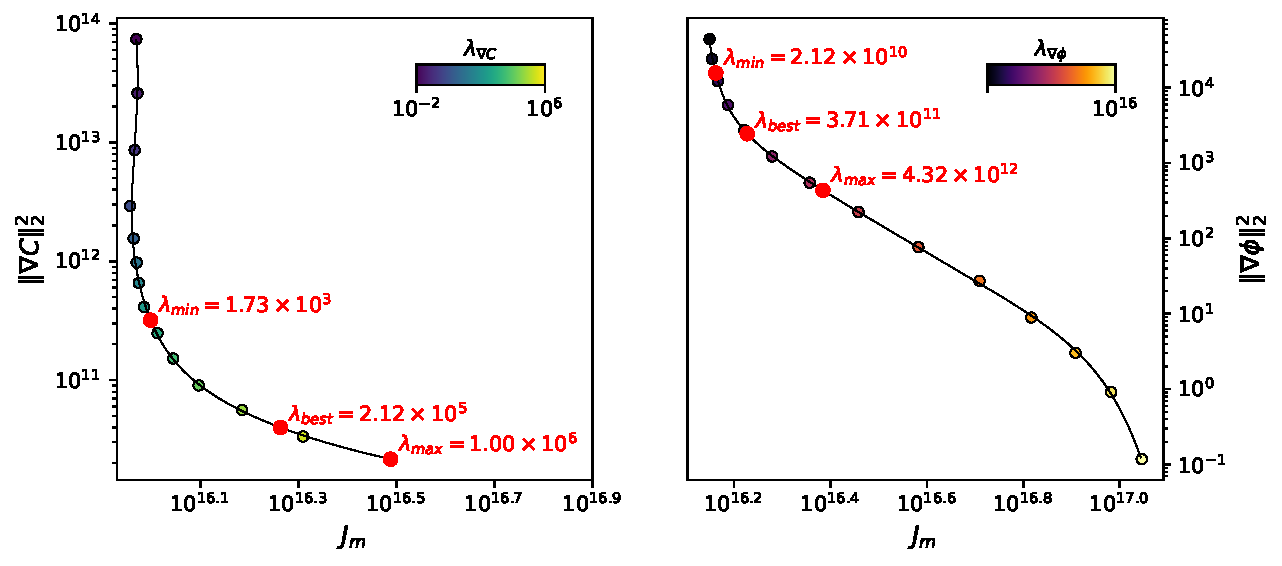
\includegraphics[width=\linewidth]{figures/lcurve.pdf}
%     \caption{L-curves}\label{fig:lcurves}
% \end{figure}

% The resulting L-curves are particularly instructive, since the corner of the L-curve is not necessarily in the location suggested by visual inspection (particularly for C). This is due to the scaling of the axes, which can easily misrepresent the curvature and is highlighted as a potential pitfall by~\cite{wolovickRegularizationLcurvesIce2023}. Equal scaling of the axes (in log-space) improves the comparison with visual inspection, but we choose to scale the axes this way due to the much larger range of values in $\log{\lvert \lvert \nabla C \rvert \rvert ^2 _2}$ compared to $\log{J_m}$, which would otherwise make it difficult to visualise the curve. This mismatch in scales can raise suspicions that the full L-curve is not sampled, but we note that higher regularisation values than those shown here cannot improve the misfit beyond the initial guess, which we take as a reasonable ceiling for regularisation strength. Our curve for C is also consistent with the L-curve in~\cite{isaacScalableEfficientAlgorithms2015}, which similarly inverts for basal friction over the Antarctic Ice Sheet. Placing this ceiling on C-regularisation also means that the L-curve is cut off before the curvature drops to half of its maximum value. In this case, we simply set $\lambda_{\text{UB}}$ to its highest possible value.

% The L-curve for $\phi$ has a similar issue with scaling, but here we can see the tail of the L-curve bending downwards as $\log \lvert \lvert \nabla \phi \rvert \rvert ^2 _2$ approaches zero, which is consistent with the idealised L-curve described in~\cite{hansenAnalysisDiscreteIllPosed1992}. In this case, it is even more clear that the different scales in the misfit and penalty terms are a real feature of the inverse problem and not of the sampling. We therefore join~\cite{wolovickRegularizationLcurvesIce2023} in strongly recommending the use of mathematical methods to determine the L-curve corner, rather than relying on visual inspection.

%%\subsection{}     %% Appendix A1, A2, etc.


\noappendix       %% use this to mark the end of the appendix section. Otherwise the figures might be numbered incorrectly (e.g. 10 instead of 1).

%% Regarding figures and tables in appendices, the following two options are possible depending on your general handling of figures and tables in the manuscript environment:

%% Option 1: If you sorted all figures and tables into the sections of the text, please also sort the appendix figures and appendix tables into the respective appendix sections.
%% They will be correctly named automatically.

%% Option 2: If you put all figures after the reference list, please insert appendix tables and figures after the normal tables and figures.
%% To rename them correctly to A1, A2, etc., please add the following commands in front of them:

\appendixfigures  %% needs to be added in front of appendix figures

\appendixtables   %% needs to be added in front of appendix tables

%% Please add \clearpage between each table and/or figure. Further guidelines on figures and tables can be found below.



\authorcontribution{TEXT} %% this section is mandatory

\competinginterests{TEXT} %% this section is mandatory even if you declare that no competing interests are present

\disclaimer{TEXT} %% optional section

\begin{acknowledgements}
TEXT
\end{acknowledgements}




%% REFERENCES

%% The reference list is compiled as follows:

% \begin{thebibliography}{}

% \bibitem[AUTHOR(YEAR)]{LABEL1}
% REFERENCE 1

% \bibitem[AUTHOR(YEAR)]{LABEL2}
% REFERENCE 2

% \end{thebibliography}

%% Since the Copernicus LaTeX package includes the BibTeX style file copernicus.bst,
%% authors experienced with BibTeX only have to include the following two lines:

\bibliographystyle{copernicus}
\bibliography{references}

%% URLs and DOIs can be entered in your BibTeX file as:
%%
%% URL = {http://www.xyz.org/~jones/idx_g.htm}
%% DOI = {10.5194/xyz}


%% LITERATURE CITATIONS
%%
%% command                        & example result
%% \citet{jones90}|               & Jones et al. (1990)
%% \citep{jones90}|               & (Jones et al., 1990)
%% \citep{jones90,jones93}|       & (Jones et al., 1990, 1993)
%% \citep[p.~32]{jones90}|        & (Jones et al., 1990, p.~32)
%% \citep[e.g.,][]{jones90}|      & (e.g., Jones et al., 1990)
%% \citep[e.g.,][p.~32]{jones90}| & (e.g., Jones et al., 1990, p.~32)
%% \citeauthor{jones90}|          & Jones et al.
%% \citeyear{jones90}|            & 1990



%% FIGURES

%% When figures and tables are placed at the end of the MS (article in one-column style), please add \clearpage
%% between bibliography and first table and/or figure as well as between each table and/or figure.

% The figure files should be labelled correctly with Arabic numerals (e.g. fig01.jpg, fig02.png).


%% ONE-COLUMN FIGURES

%%f
%\begin{figure}[t]
%\includegraphics[width=8.3cm]{FILE NAME}
%\caption{TEXT}
%\end{figure}
%
%%% TWO-COLUMN FIGURES
%
%%f
%\begin{figure*}[t]
%\includegraphics[width=12cm]{FILE NAME}
%\caption{TEXT}
%\end{figure*}
%
%
%%% TABLES
%%%
%%% The different columns must be seperated with a & command and should
%%% end with \\ to identify the column brake.
%
%%% ONE-COLUMN TABLE
%
%%t
%\begin{table}[t]
%\caption{TEXT}
%\begin{tabular}{column = lcr}
%\tophline
%
%\middlehline
%
%\bottomhline
%\end{tabular}
%\belowtable{} % Table Footnotes
%\end{table}
%
%%% TWO-COLUMN TABLE
%
%%t
%\begin{table*}[t]
%\caption{TEXT}
%\begin{tabular}{column = lcr}
%\tophline
%
%\middlehline
%
%\bottomhline
%\end{tabular}
%\belowtable{} % Table Footnotes
%\end{table*}
%
%%% LANDSCAPE TABLE
%
%%t
%\begin{sidewaystable*}[t]
%\caption{TEXT}
%\begin{tabular}{column = lcr}
%\tophline
%
%\middlehline
%
%\bottomhline
%\end{tabular}
%\belowtable{} % Table Footnotes
%\end{sidewaystable*}
%
%
%%% MATHEMATICAL EXPRESSIONS
%
%%% All papers typeset by Copernicus Publications follow the math typesetting regulations
%%% given by the IUPAC Green Book (IUPAC: Quantities, Units and Symbols in Physical Chemistry,
%%% 2nd Edn., Blackwell Science, available at: http://old.iupac.org/publications/books/gbook/green_book_2ed.pdf, 1993).
%%%
%%% Physical quantities/variables are typeset in italic font (t for time, T for Temperature)
%%% Indices which are not defined are typeset in italic font (x, y, z, a, b, c)
%%% Items/objects which are defined are typeset in roman font (Car A, Car B)
%%% Descriptions/specifications which are defined by itself are typeset in roman font (abs, rel, ref, tot, net, ice)
%%% Abbreviations from 2 letters are typeset in roman font (RH, LAI)
%%% Vectors are identified in bold italic font using \vec{x}
%%% Matrices are identified in bold roman font
%%% Multiplication signs are typeset using the LaTeX commands \times (for vector products, grids, and exponential notations) or \cdot
%%% The character * should not be applied as mutliplication sign
%
%
%%% EQUATIONS
%
%%% Single-row equation
%
%\begin{equation}
%
%\end{equation}
%
%%% Multiline equation
%
%\begin{align}
%& 3 + 5 = 8\\
%& 3 + 5 = 8\\
%& 3 + 5 = 8
%\end{align}
%
%
%%% MATRICES
%
%\begin{matrix}
%x & y & z\\
%x & y & z\\
%x & y & z\\
%\end{matrix}
%
%
%%% ALGORITHM
%
%\begin{algorithm}
%\caption{...}
%\label{a1}
%\begin{algorithmic}
%...
%\end{algorithmic}
%\end{algorithm}
%
%
%%% CHEMICAL FORMULAS AND REACTIONS
%
%%% For formulas embedded in the text, please use \chem{}
%
%%% The reaction environment creates labels including the letter R, i.e. (R1), (R2), etc.
%
%\begin{reaction}
%%% \rightarrow should be used for normal (one-way) chemical reactions
%%% \rightleftharpoons should be used for equilibria
%%% \leftrightarrow should be used for resonance structures
%\end{reaction}
%
%
%%% PHYSICAL UNITS
%%%
%%% Please use \unit{} and apply the exponential notation (e.g. 20\,\unit{W\,m^{-2}})


\end{document}
